\chapter{Procurement Evaluation Methodology}
\section{Make-or-Buy Decision Framing}
The choice between in-house software development and commercial SaaS platforms comes down to balancing recurring subscription costs against internal development and maintenance responsibilities. Every formal software procurement evaluates these two core paths:
\begin{itemize}[itemsep=1pt,topsep=1pt]
    \item \textbf{Internal Construction and Ownership ("Make")}: Eliminates per-seat subscription royalties and preserves full control over source code, data residency, offline execution, and custom \textbf{PMBOK\textsuperscript{\textregistered} Guide (Chapter 6)} scheduling algorithms \cite{pmbok}. In return, the organization must self-fund security hardening, hosting, maintenance, and future features.
    \item \textbf{Commercial Off-the-Shelf Licensing ("Buy")}: Delivers mature enterprise modules, uptime Service Level Agreements, managed security, and external support immediately. In return, the buyer accepts recurring per-seat royalties, renewal price increases, and external product roadmaps.
\end{itemize}

\vspace{2mm}

\noindent This report evaluates that choice across a standardized \textbf{25-user team over 36 months} (3 Project Managers, 2 Controllers, and 20 Team Members). A €0 license fee reflects internal ownership custody, not free deployment or permanent zero-price SaaS positioning. Because tools target distinct workflows across \textbf{Waterfall}, \textbf{Agile}, and \textbf{Hybrid} teams, our evaluation balances delivery-model fairness alongside predictive schedule rigor.

\vspace{8mm}

\section{Structured Source Selection Workflow}
Locking all screening gates, weights, and cost formulas before inspecting any product prevents post-hoc bias. The six-stage workflow below structures the rest of this document:

\begin{figure}[H]
    \centering
    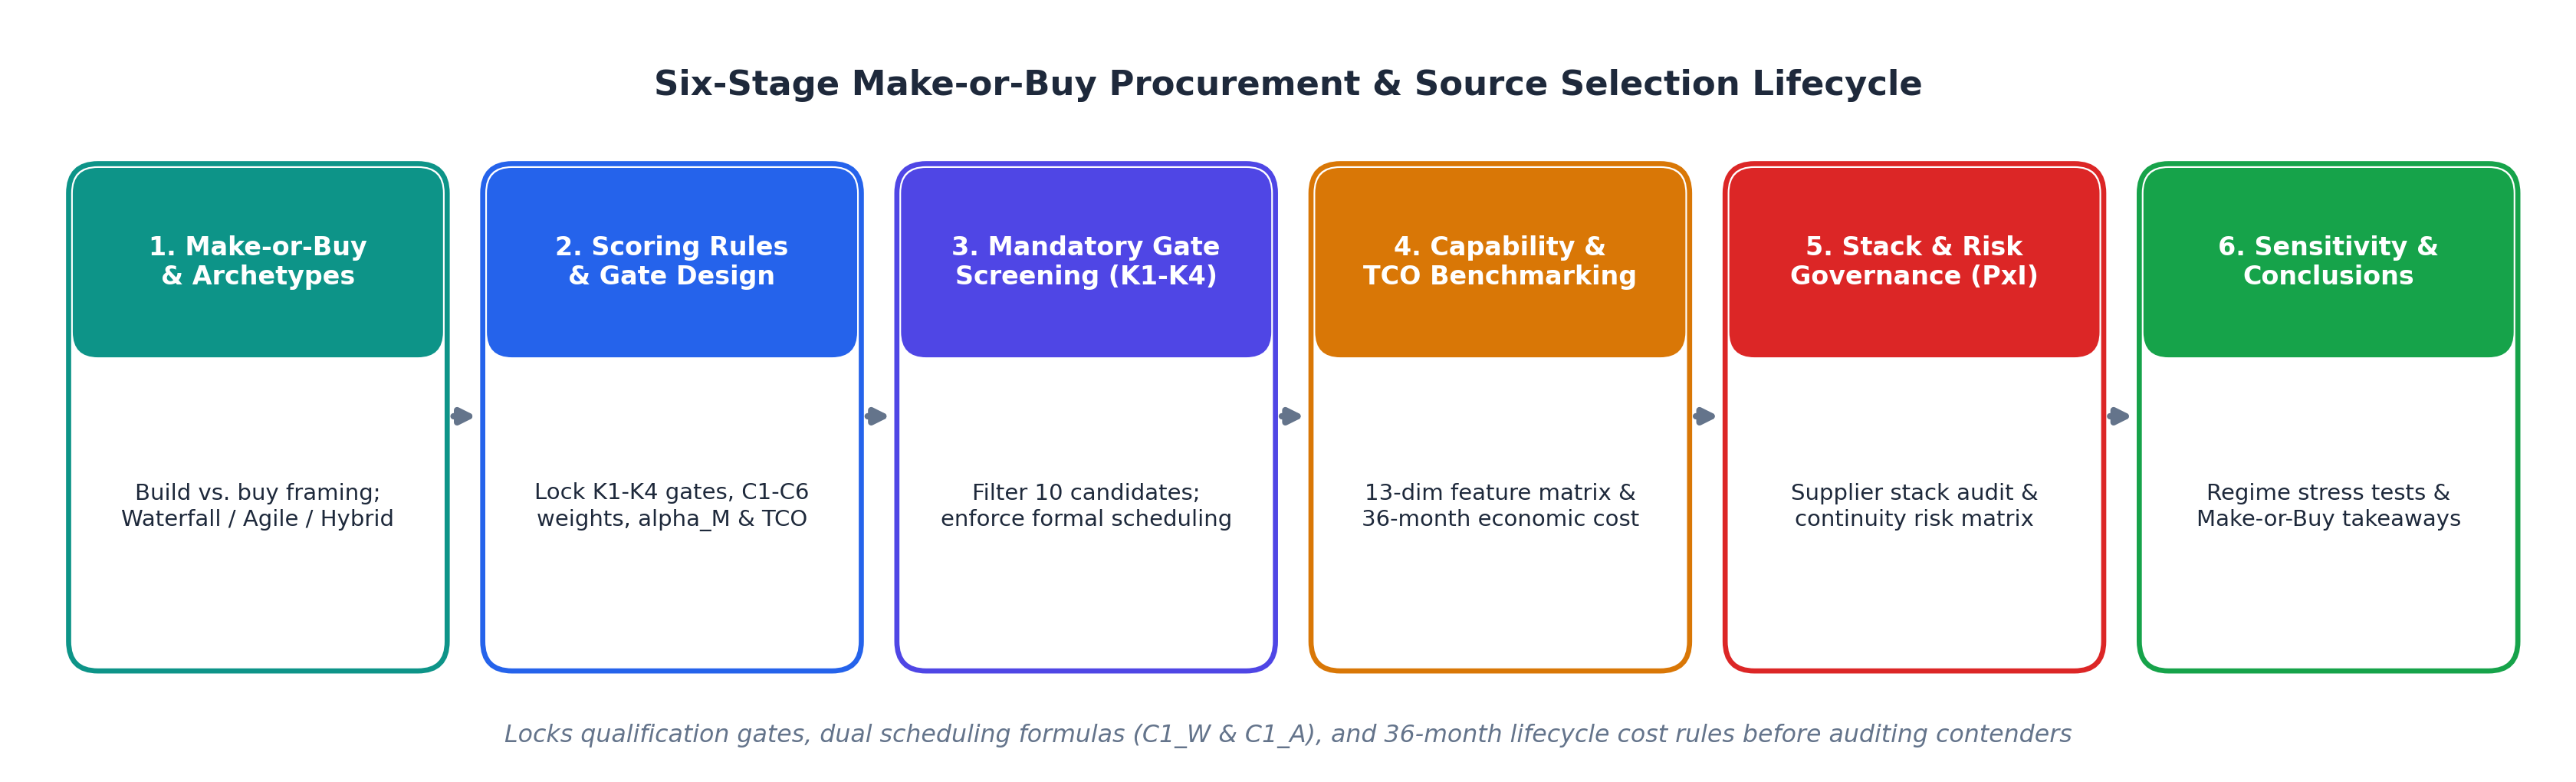
\includegraphics[width=1.0\textwidth]{images/va_process_flow.png}
    \caption*{Six-stage Make-or-Buy procurement and source-selection workflow linking methodology lock, screening, benchmarking, risk governance, and conclusions.}
\end{figure}

\newpage

\noindent Each stage maps to a subsequent section of this analysis:
\begin{enumerate}[leftmargin=2.2em,labelsep=0.5em,itemsep=1pt,topsep=1pt]
	\item \textbf{Framing and Archetype Rules (Chapter 2)}: Define the Make-or-Buy scope, delivery paradigms, pass/fail gates ($K_1$--$K_4$), scoring criteria ($C_1$--$C_6$), and 36-month TCO equations;
	\item \textbf{Market Candidate Screening (Chapter 3.1)}: Apply gates $K_1$--$K_4$ to all ten initial candidates, retaining only tools meeting baseline scheduling requirements;
	\item \textbf{Capability Audit, Rankings, and TCO (Chapters 3.2--3.6)}: Assess qualifying contenders across thirteen capabilities, compute three-year lifecycle costs and metrics, and rank baseline \textit{v1.0} and projected \textit{v2.0} tiers;
	\item \textbf{Make-Candidate Supply-Chain Audit (Chapter 4)}: Audit external cloud APIs, databases, backend frameworks, frontend visualization packages, and orchestration tools supporting the internal "Make" candidate;
	\item \textbf{Supply-Chain Risk and Sensitivity Governance (Chapter 5)}: Assess vendor lock-in, maintainer continuity, privacy, and hardening risks ($P \times I$), alongside ranking stability under alternative stakeholder priorities;
	\item \textbf{Conclusions (Chapter 6)}: Summarize methodology-aware rankings, current baseline boundaries, and projected \textit{SyncFlow v2.0} upgrade outcomes.
\end{enumerate}


\vspace{4mm}

\section{Delivery Methodology Classification}
Because schedule management tools reflect distinct project management philosophies, each candidate entering the screening funnel is classified into one of three foundational archetypes ($\mathcal{M}_i \in \{\text{Waterfall}, \text{Agile}, \text{Hybrid}\}$):
\begin{itemize}[itemsep=1pt,topsep=1pt]
	\item \textbf{Waterfall ($\text{W}$, Predictive)}: Based on hierarchical WBS baselines, precedence networks (\texttt{FS/SS/FF/SF} with lags), Critical Path float analysis, EVM baselines, and formal schedule audits;
	\item \textbf{Agile ($\text{A}$, Iterative Velocity Flow)}: Based on prioritized product backlogs, fixed-length sprints or continuous WIP boards, story-point velocity forecasting, burndowns, and CI/CD release streams;
	\item \textbf{Hybrid ($\text{H}$, Dual-Mode Convergence)}: Combines predictive planning (WBS trees, Gantt dependencies, milestone baselines) with iterative execution workflows, status-pull boards, or Scrum sprints.
\end{itemize}

\vspace{4mm}

\section{Knockout Qualification Gates}
Four binary pass/fail gates filter out lightweight task lists before detailed scoring begins. Every candidate must satisfy all four \textbf{Knockout Gates} ($K_1$--$K_4$):
\begin{itemize}[itemsep=1pt,topsep=1pt]
    \item \textbf{Gate $K_1$ (Structured Activity Relations)}: Must model explicit activity dependencies, sprint backlog hierarchies, or blocked-by release relationships, not standalone task cards;
    \item \textbf{Gate $K_2$ (Formal Schedule Forecasting)}: Must support critical-path float calculations, velocity-based sprint forecasts, or cross-team milestone warnings, natively or via ecosystem add-ons;
    \item \textbf{Gate $K_3$ (Collaborative Multi-User Access)}: Must coordinate multiple assigned team roles across shared workspaces;
    \item \textbf{Gate $K_4$ (Auditable Cost Visibility)}: Must provide published list rates, transparent enterprise quote structures, or verifiable internal hosting and labor estimates.
\end{itemize}

\newpage

\section{Paradigm-Normalized Scoring System}
The scoring model maps half-point human ratings and audited three-year costs onto a bounded $[0, 5]$ scale via five sequential equations. Each qualitative criterion uses a structured \textbf{half-point ($0.5$-increment) anchored scale} drawn from $\mathcal{D} = \{0, 0.5, 1.0, \dots, 5.0\} \subset [0, 5]$ (with $0.0$ and $0.5$ reserved when a required feature is absent). Six integer milestone anchors calibrate these votes:
\begin{itemize}[itemsep=1pt,topsep=1pt]
    \item \textbf{0 (Absent / Non-Compliant)}: Required capability or control is absent from the platform;
    \item \textbf{1 (Manual Workaround)}: Core workflow can only be approximated externally through manual spreadsheets, custom scripting, or offline workarounds;
    \item \textbf{2 (Partial / Limited)}: Basic support is present in simplified form, omitting algorithmic depth, automation, or multi-user controls;
    \item \textbf{3 (Standard Commercial Fit)}: Meets standard day-to-day industry expectations reliably with solid baseline capabilities;
    \item \textbf{4 (Strong Professional Grade)}: Provides mature, well-integrated, high-reliability functionality suited to demanding project environments;
    \item \textbf{5 (Best-in-Class Reference)}: Sets the cohort benchmark in mathematical rigor, workflow coverage, security governance, or cost efficiency.
\end{itemize}

\noindent Financial efficiency ($C_6$) and the combined summary indices ($C_1^*$, $Q_{\text{fair}}$, $S_{\text{fair}}$, $S_{\text{CPM}}$) are real-valued outputs computed deterministically from explicit formulas. Across the full evaluation vector, each criterion $C_j$ carries a strictly positive weight $w_j > 0$ forming a normalized distribution ($\sum_{j=1}^{6} w_j = 1.00$):

\begin{table}[H]
\centering
\footnotesize
\setlength{\tabcolsep}{4.5pt}
\renewcommand{\arraystretch}{1.15}
\begin{tabularx}{\textwidth}{>{\raggedright\arraybackslash}p{4.5cm} c >{\raggedright\arraybackslash}X}
\toprule
\textbf{Evaluation Dimension} & \textbf{Weight ($w_j$)} & \textbf{Audit Scope} \\
\midrule
$C_1$: Scheduling Engine Performance & $0.25$ & Methodology-normalized blend $C_1^*$ combining Predictive OR math ($C_{1,W}$) and Agile iterative flow ($C_{1,A}$). \\
$C_2$: Suite Breadth (Cost, Risk) & $0.15$ & Monetary budgets/billing rates, Risk Registers, resource leveling, RACI tabs, cross-project rollups, rich integrations. \\
$C_3$: AI, Usability \& Interoperability & $0.15$ & Generative AI schedule drafting, role-based persona UX, learning curve friction, REST APIs, \texttt{.mpp}/\texttt{.xml}/\texttt{CSV} or Git/DevOps sync. \\
$C_4$: Vendor Maturity, Security, SLA & $0.15$ & Backed uptime SLAs, SAML SSO/SCIM, compliance certifications, TLS defaults, auth recovery flows, automated CI tests. \\
$C_5$: Autonomy, Extensibility & $0.10$ & Data residency control, open-source auditability, zero vendor lock-in, customizable algorithmic core. \\
$C_6$: 3-Year TCO Efficiency & $0.20$ & Formulaic log-normalized 36-month economic cost across SaaS seats, hosting, hardening, upgrades, and maintenance. \\
\bottomrule
\end{tabularx}
\end{table}

\vspace{2mm}

In plain terms, a single weighted average can still behave unfairly if it forces an Agile sprint platform and a Waterfall platform onto identical scheduling rules, or if low licensing prices hide weak technical quality. The scoring function solves both issues through five sequential, mathematically closed transformations that keep every derived score inside the $[0, 5]$ interval:

\begin{enumerate}[leftmargin=2.2em,labelsep=0.5em,itemsep=1.5pt,topsep=1pt]
\setlength{\abovedisplayskip}{4pt}
\setlength{\belowdisplayskip}{4pt}
    \item \textbf{Step 1: Splitting Scheduling Performance Into Two Tracks ($C_{1,W}$ and $C_{1,A}$)}. Criterion $C_1$ accounts for one quarter of the total score ($w_1 = 0.25$). Instead of collapsing all scheduling behavior into one grade, each platform $i$ receives two separate half-point ratings on $[0, 5]$:
    \begin{itemize}[itemsep=1pt,topsep=1pt]
        \item \textbf{Predictive Waterfall Rigor ($C_{1,W,i}$)}: Measures formal PDM dependency networks, CPM float math, PERT probability curves, EVM baselines, and DCMA schedule checks;
        \item \textbf{Agile Iterative Flow ($C_{1,A,i}$)}: Measures Scrum backlogs, story points, velocity forecasting, burndown charts, WIP pull workflows, and CI/CD release links.
    \end{itemize}
	\newpage
    \item \textbf{Step 2: Convex Blending via Delivery Archetype ($C_{1,i}^*$)}. To reflect what each software product was actually designed to do without ignoring structural dependencies, $C_{1,i}^*$ is formed as a \textbf{convex linear combination} of $C_{1,W,i}$ and $C_{1,A,i}$ parameterized by an archetype coefficient $\alpha_{\mathcal{M}_i} \in [0.30, 0.85]$:
    $$
        C_{1,i}^* = \alpha_{\mathcal{M}_i}\, C_{1,W,i} + (1 - \alpha_{\mathcal{M}_i})\, C_{1,A,i} \qquad \qquad
        \alpha_{\mathcal{M}_i} = \begin{cases}
            0.85 & \text{if } \mathcal{M}_i = \text{Waterfall,} \\
            0.60 & \text{if } \mathcal{M}_i = \text{Hybrid,} \\
            0.30 & \text{if } \mathcal{M}_i = \text{Agile.}
        \end{cases}
    $$
    Mathematically, because $\alpha_{\mathcal{M}_i} \in (0, 1)$ and both sub-scores lie in $[0, 5]$, their convex combination $C_{1,i}^*$ is bounded strictly between $\min(C_{1,W,i}, C_{1,A,i})$ and $\max(C_{1,W,i}, C_{1,A,i})$, preserving the $[0, 5]$ codomain cleanly. To ensure calculation transparency, intermediate blended scores $C_{1,i}^*$ are rounded to two decimal places ($\text{round}_2$, e.g., for TeamGantt: $0.85(3.5) + 0.15(2.0) = 3.275 \to \mathbf{3.28}$) before entering composite formulas. Final summary metrics ($Q_{\text{fair}}, S_{\text{fair}}, S_{\text{CPM}}$) are likewise rounded to two decimal places, ensuring invariance to floating-point precision artifacts. Substantively, the coefficients never reach $0$ or $1$: Waterfall tools keep a $15\%$ iterative check ($3.75\%$ overall), Hybrid tools balance $60\%$ predictive / $40\%$ agile ($15\%$ and $10\%$ overall), and Agile tools keep a $30\%$ structural dependency floor ($7.50\%$ predictive vs. $17.50\%$ agile overall) so cross-team milestone logic is never ignored;

    \item \textbf{Step 3: Weighted Composite Score ($S_{\text{fair},i}$)}. Combining all six criteria yields a continuous, strictly monotonic linear functional over the product domain $[0, 5]^6$ directly serving as the headline \textbf{Paradigm-Fair Score}:
    $$
        S_{\text{fair},i} = w_1 C_{1,i}^* + \sum_{j=2}^{6} w_j s_{i,j} = 0.25\, C_{1,i}^* + 0.15\, s_{i,2} + 0.15\, s_{i,3} + 0.15\, s_{i,4} + 0.10\, s_{i,5} + 0.20\, s_{i,6}.
    $$
    Because all weights are strictly positive ($\partial S_{\text{fair},i} / \partial s_{i,j} = w_j > 0$) and sum to $1.00$, $S_{\text{fair},i}$ is a normalized convex average bounded inside $[0, 5]$: improving any single dimension strictly raises the total score, while scoring $4.0$ across every dimension yields exactly $S_{\text{fair},i} = 4.0$. Note that $s_{i,6} \in [0.5, 5.0]$ comes from the smooth bounded logarithmic cost function defined in Section 2.6;

    \item \textbf{Step 4: Orthogonal Decomposition to Isolate Pure Technical Quality ($Q_{\text{fair},i}$)}. Before considering money, decision makers need to see whether a cheap product is genuinely capable. Splitting $S_{\text{fair},i}$ into its technical component ($w_1 + \dots + w_5 = 0.80$) and its cost component ($w_6 = 0.20$) gives $S_{\text{fair},i} = 0.80\, Q_{\text{fair},i} + 0.20\, s_{i,6}$, where pure \textbf{Paradigm-Fair Quality} is rescaled back onto $[0, 5]$ by dividing through by $0.80$:
    $$
        Q_{\text{fair},i} = \frac{w_1 C_{1,i}^* + \sum_{j=2}^{5} w_j s_{i,j}}{0.80}
        = 0.3125\, C_{1,i}^* + 0.1875\,(s_{i,2} + s_{i,3} + s_{i,4}) + 0.1250\, s_{i,5}.
    $$
    Notice that the normalized weights $(0.3125, 0.1875, 0.1875, 0.1875, 0.1250)$ again sum to $1.00$. Separating $Q_{\text{fair},i}$ completely from $s_{i,6}$ prevents circular reasoning when Chapter 3 plots technical quality directly against three-year cost and computes cost per quality point ($\text{TCO}_{3\text{yr},i} / Q_{\text{fair},i}$).

    \item \textbf{Step 5: The Strict Predictive Boundary Case ($S_{\text{CPM},i}$)}. Alongside $S_{\text{fair},i}$, the framework evaluates a parallel boundary case, the \textbf{Strict Predictive PMBOK-CPM Benchmark ($S_{\text{CPM},i}$)}, obtained by setting $\alpha_{\mathcal{M}_i} \equiv 1$ across all candidates ($C_{1,i}^* \to C_{1,W,i}$) and updating cost ($s_{i,6,\text{cpm}}$) wherever external add-on plugins are required to supply critical-path math:
    $$
        S_{\text{CPM},i} = w_1 C_{1,W,i} + \sum_{j=2}^{5} w_j s_{i,j} + w_6 s_{i,6,\text{cpm}}
    $$
    Comparing the two lenses yields a direct linear identity when $s_6$ stays fixed: the score difference $S_{\text{fair},i} - S_{\text{CPM},i} = w_1\, (1 - \alpha_{\mathcal{M}_i})\, (C_{1,A,i} - C_{1,W,i})$ equals the exact product of the paradigm relaxation $(1 - \alpha_{\mathcal{M}_i})$ and the Agile-versus-Waterfall gap $(C_{1,A,i} - C_{1,W,i})$. 
\end{enumerate}

\newpage

\section{Lifecycle Cost Modeling}
Three-year Total Cost of Ownership captures both direct subscriptions and full internal engineering labor on one standardized 25-user, 36-month baseline ($t = 36$, $1\text{ USD} = 0.92\text{ EUR}$):
\begin{equation*}
    \setlength{\abovedisplayskip}{3pt}
    \setlength{\belowdisplayskip}{3pt}
    \text{TCO}_{3\text{yr},i} = C_{\text{license}} + C_{\text{infra/API}} + C_{\text{deploy}} + C_{\text{future}} + C_{\text{maint}}
\end{equation*}
Five cost components prevent hidden subsidies when comparing cloud SaaS subscriptions against self-hosted software:
\begin{itemize}[itemsep=0.5pt,topsep=1pt,parsep=0pt]
    \item \textbf{$C_{\text{license}}$ (Software Licenses)}: Three-year SaaS subscription fees (€0 under internal Make ownership, treating prior prototype work as sunk R\&D);
    \item \textbf{$C_{\text{infra/API}}$ (Infrastructure and AI APIs)}: VPS hosting, automated off-site backups, DNS/SMTP email, and paid AI API reserves (€0 where SaaS bundles hosting);
    \item \textbf{$C_{\text{deploy}}$ (Deployment, Hardening, and Onboarding)}: Initial SaaS onboarding, user provisioning, and SSO configuration, or internal pre-rollout security hardening (standardized at 36 hours across vendors);
    \item \textbf{$C_{\text{future}}$ (Planned Upgrade Engineering at €45/Hour)}: Internal EU ICT labor benchmark \cite{eurostat} funding all planned \textit{SyncFlow v2.0} enhancements (defined in Section 3.6), plus CPM plugins under Strict PMBOK audits;
    \item \textbf{$C_{\text{maint}}$ (Ongoing Administration)}: Routine administration, dependency patching, and user support across 36 months.
\end{itemize}

\vspace{1mm}

\noindent \textbf{Accounting Treatment: Sunk R\&D Costs vs. Greenfield Counterfactual}. A critical reviewer might ask: \textit{"Why is the development effort to create SyncFlow v1.0 considered free ($C_{\text{license}} = \text{€}0$), while commercial rivals incur license fees from day one? If an organization were to build SyncFlow from scratch, it would also have to pay for those initial development hours!"}

To resolve this question rigorously, the procurement audit distinguishes between four precise project lifecycle dimensions:
\begin{itemize}[itemsep=1pt,topsep=1pt]
    \item \textbf{Calendar Duration ($T_{\text{cal}}$)}: Total project window spanning \textbf{53 calendar days} (September 21 to November 13). As documented in the project milestone ledger, this timeline absorbs an initial ideation phase, an unforeseen 5-day pause (\textit{force majeure}, Sep 25--29), 6 scheduled rest days, post-software documentation (Nov 10--11), and preparation of the Vendor Analysis itself (Nov 12--13). Crucially, the software codebase was completed and frozen on \textbf{November 9} (a 50-calendar-day span);
    \item \textbf{Active Development Days ($D_{\text{act}}$)}: Days strictly dedicated to software engineering. Deducting the 5-day pause, 6 scheduled rest days, the unlogged Nov 8 gap, the November 9 project sign-off, and the 4 post-software documentation and analysis days ($53 - 5 - 6 - 1 - 1 - 4 = 36$) yields exactly \textbf{36 active development days} dedicated to architecture, database schemas, OR algorithms, DCMA audit checks, and frontend UI refactoring;
    \item \textbf{Estimated Historical Development Effort ($H_{\text{eng}}$)}: Reconstructed engineering effort. In the absence of granular automated timesheets during development, the 252 hours represent a reconstructed estimate rather than an actually measured figure (informal estimates of 300--400 hours cannot be cited as documented data). Instead, historical development effort is modeled by anchoring on the \textbf{252 engineering hours} established in our screening audit (Table 3.1), reflecting $36\text{ active days} \times 7\text{ hours/day} = 252\text{ hours}$ of focused technical labor;
    \item \textbf{Economic Development Cost ($C_{\text{dev}}$)}: Economic value of the reconstructed hours, evaluated at the standard EU ICT labor benchmark rate ($w_h = \text{€}45/\text{h}$ \cite{eurostat}):
    \begin{equation*}
        C_{\text{dev}} = 252\text{h} \times \text{€}45/\text{h} = \textbf{€11,340}
    \end{equation*}
\end{itemize}

Under managerial accounting standards (PMBOK Guide, Section 2.8, IFRS/GAAP IAS 38), this historical €11,340 represents an unrecoverable \textbf{sunk cost} at the procurement decision point: it cannot be recovered whether \textit{SyncFlow} or a commercial tool is deployed. Therefore, in forward-looking cash flow modeling, the marginal license cost of an existing internal asset is strictly $C_{\text{license}} = \text{€}0$ and baseline upgrade effort is $C_{\text{future}} = \text{€}0$, leaving only operational cash flows: hosting, hardening, and maintenance ($\text{TCO}_{\text{v1.0}} = \textbf{€6,492}$).

Conversely, an organization evaluating a greenfield "Make-from-scratch" build must treat $C_{\text{dev}} = \text{€}11,340$ as upfront CapEx ($C_{\text{initial}}$), yielding a total greenfield build-and-run lifecycle cost of:
\begin{equation*}
    \text{TCO}_{\text{greenfield, v1.0}} = \text{€}11,340 + \text{€}6,492 = \textbf{€17,832}
\end{equation*}
matching mid-tier commercial suites (e.g. \textit{Jira Premium} at €17,084). For \textit{SyncFlow v2.0}, the 400 engineering hours ($C_{\text{future}} = \text{€}18,000$) represent new, uncommitted future labor, correctly charged to $\text{TCO}_{\text{v2.0}} = \textbf{€24,492}$.

\vspace{1mm}

\noindent \textbf{Three-Scenario Strategic Procurement Framework}. To ensure analytical transparency and prevent conflating the economic advantage of an existing prototype with the inherent viability of the software architecture, the evaluation formally distinguishes three separate, clearly labeled procurement scenarios:

\begin{table}[H]
\centering
\scriptsize
\setlength{\tabcolsep}{3.5pt}
\renewcommand{\arraystretch}{1.18}
\caption*{Strategic Procurement Framework: Make vs. Buy Decision Contexts.}
\begin{tabularx}{\textwidth}{>{\bfseries}l >{\raggedright}X >{\raggedright}X c c}
\toprule
Scenario & Decision Context \& Operational Status & Accounting Treatment \& Scope & 3-Yr TCO & $C_6$ \\
\midrule
Make -- Existing Asset & SyncFlow is already developed. Only future operational costs are considered. & Forward-looking OpEx only. €11,340 historical R\&D treated as sunk. & \textbf{€6,492} & \textbf{5.0} \\
Make -- Greenfield & The organization must develop SyncFlow from scratch without existing assets. & Full lifecycle: €11,340 upfront CapEx plus €6,492 3-year run cost. & \textbf{€17,832} & \textbf{4.2} \\
Buy -- Commercial Solution & The organization purchases an existing, commercially available turnkey solution. & Multi-year commercial subscription fees plus deployment and hosting. & \textbf{€8,655--€137,500} & \textbf{1.9--5.0} \\
\bottomrule
\end{tabularx}
\end{table}

\vspace{1mm}

Raw three-year costs convert into a $0.5\text{--}5.0$ cost score ($s_{i,6}$) via Base-10 logarithmic scaling against $\text{TCO}_{\text{ref}}$, the \textbf{lowest qualifying commercial vendor TCO} established in Chapter 3:
\begin{equation*}
    \setlength{\abovedisplayskip}{3pt}
    \setlength{\belowdisplayskip}{3pt}
    s_{i,6} = \text{round}_1\!\left(\min\!\left(5.0,\;\max\!\left(0.5,\; 5.0 - 2.6 \cdot \log_{10}\!\left(\frac{\text{TCO}_{3\text{yr},i}}{\text{TCO}_{\text{ref}}}\right)\right)\right)\right)
\end{equation*}
Crucially, the raw continuous output of the cost equation is explicitly rounded to one decimal place ($\text{round}_1$) to produce the criterion rating $s_{i,6}$ before it is introduced into the composite equations ($S_{\text{fair}}$ and $S_{\text{CPM}}$). This rounding convention ensures consistency with the calibrated half-point and single-decimal granularity of the qualitative criteria ($C_1\text{--}C_5$), preventing infinitesimal pricing variations from dominating multi-criteria rankings.

Because software costs span a tenfold range (below €10,000 to over €100,000), linear scaling compresses mid-tier options toward zero. Log scaling preserves fair sensitivity: matching $\text{TCO}_{\text{ref}}$ scores $5.0$, doubling cost ($2\times \text{TCO}_{\text{ref}}$) drops $s_{i,6}$ to $4.22 \to 4.2$, a tenfold cost scores $2.40 \to 2.4$, and the $0.50$ floor keeps extreme enterprise tiers positive.
